\documentclass[letterpaper,11pt,twoside,]{pinp}

%% Some pieces required from the pandoc template
\providecommand{\tightlist}{%
  \setlength{\itemsep}{0pt}\setlength{\parskip}{0pt}}

% Use the lineno option to display guide line numbers if required.
% Note that the use of elements such as single-column equations
% may affect the guide line number alignment.

\usepackage[T1]{fontenc}
\usepackage[utf8]{inputenc}
\usepackage{longtable}

% pinp change: the geometry package layout settings need to be set here, not in pinp.cls
\geometry{layoutsize={0.95588\paperwidth,0.98864\paperheight},%
  layouthoffset=0.02206\paperwidth, layoutvoffset=0.00568\paperheight}

\definecolor{pinpblue}{HTML}{185FAF}  % imagecolorpicker on blue for new R logo
\definecolor{pnasbluetext}{RGB}{101,0,0} %



\title{Lab 005 - Inference for means - Solutions}

\author[a]{EPIB607 - Inferential Statistics}

  \affil[a]{McGill University}

\setcounter{secnumdepth}{5}

% Please give the surname of the lead author for the running footer
\leadauthor{Bhatnagar and Hanley}

% Keywords are not mandatory, but authors are strongly encouraged to provide them. If provided, please include two to five keywords, separated by the pipe symbol, e.g:
 \keywords{  Sampling distribution |  Standard error |  Normal
distribution |  Quantiles |  Percentiles |  Z-scores  }  

\begin{abstract}
In this exercise you will practice calculating confidence intervals
using the t-distribution and the bootstrap.
\end{abstract}

\dates{This version was compiled on \today} 

% initially we use doi so keep for backwards compatibility
\doifooter{\url{https://sahirbhatnagar.com/EPIB607/}}
% new name is doi_footer

\pinpfootercontents{Lab 005}

\begin{document}

% Optional adjustment to line up main text (after abstract) of first page with line numbers, when using both lineno and twocolumn options.
% You should only change this length when you've finalised the article contents.
\verticaladjustment{-2pt}

\maketitle
\thispagestyle{firststyle}
\ifthenelse{\boolean{shortarticle}}{\ifthenelse{\boolean{singlecolumn}}{\abscontentformatted}{\abscontent}}{}

% If your first paragraph (i.e. with the \dropcap) contains a list environment (quote, quotation, theorem, definition, enumerate, itemize...), the line after the list may have some extra indentation. If this is the case, add \parshape=0 to the end of the list environment.


\begin{longtable}[]{@{}ll@{}}
\toprule
R Code & Value \\
\midrule
\endhead
\texttt{qnorm(p\ =\ c(0.05,\ 0.95))} & -1.64, 1.64 \\
\texttt{qnorm(p\ =\ c(0.025,\ 0.975))} & -1.96, 1.96 \\
\texttt{qnorm(p\ =\ c(0.005,\ 0.995))} & -2.58, 2.58 \\
\texttt{qt(p\ =\ c(0.025,\ 0.975),\ df\ =\ 400-1)} & -1.97, 1.97 \\
\texttt{qt(p\ =\ c(0.025,\ 0.975),\ df\ =\ 25-1)} & -2.06, 2.06 \\
\texttt{qt(p\ =\ c(0.025,\ 0.975),\ df\ =\ 20-1)} & -2.09, 2.09 \\
\texttt{qt(p\ =\ c(0.025,\ 0.975),\ df\ =\ 16-1)} & -2.13, 2.13 \\
\bottomrule
\end{longtable}

\hypertarget{food-intake-and-weight-gain}{%
\section{Food intake and weight
gain}\label{food-intake-and-weight-gain}}

If we increase our food intake, we generally gain weight. Nutrition
scientists can calculate the amount of weight gain that would be
associated with a given increase in calories. In one study, 16 nonobese
adults, aged 25 to 36 years, were fed 1000 calories per day in excess of
the calories needed to maintain a stable body weight. The subjects
maintained this diet for 8 weeks, so they consumed a total of 56,000
extra calories. According to theory, 3500 extra calories will translate
into a weight gain of 1 pound. Therfore we expect each of these subjects
to gain 56,000/3500=16 pounds (lb). Here are the weights (given in the
\texttt{weightgain.csv} file) before and after the 8-week period
expressed in kilograms (kg):

\begin{Shaded}
\begin{Highlighting}[]
\NormalTok{weight }\OtherTok{\textless{}{-}} \FunctionTok{read.csv}\NormalTok{(}\StringTok{"weightgain.csv"}\NormalTok{)}
\end{Highlighting}
\end{Shaded}

\begin{enumerate}
\def\labelenumi{\alph{enumi}.}
\tightlist
\item
  Calculate a 95\% confidence interval for the mean weight change and
  give a sentence explaining the meaning of the 95\%. State your
  assumptions.
\end{enumerate}

\begin{Shaded}
\begin{Highlighting}[]
\NormalTok{weight }\OtherTok{\textless{}{-}} \FunctionTok{read.csv}\NormalTok{(}\StringTok{"\textasciitilde{}/git\_repositories/epib607/inst/labs/005{-}one{-}sample{-}mean/weightgain.csv"}\NormalTok{)}

\CommentTok{\# Creating new variable for weight change}
\NormalTok{weight}\SpecialCharTok{$}\NormalTok{change }\OtherTok{\textless{}{-}}\NormalTok{ weight}\SpecialCharTok{$}\NormalTok{after}\SpecialCharTok{{-}}\NormalTok{weight}\SpecialCharTok{$}\NormalTok{before}
\NormalTok{weight}\SpecialCharTok{$}\NormalTok{change\_lb }\OtherTok{\textless{}{-}}\NormalTok{ weight}\SpecialCharTok{$}\NormalTok{change}\SpecialCharTok{*}\FloatTok{2.2}

\CommentTok{\# Calculating the mean of weight change and rounding}
\NormalTok{(ybar\_change }\OtherTok{\textless{}{-}} \FunctionTok{mean}\NormalTok{(weight}\SpecialCharTok{$}\NormalTok{change))}
\end{Highlighting}
\end{Shaded}

\begin{ShadedResult}
\begin{verbatim}
#  [1] 4.7
\end{verbatim}
\end{ShadedResult}

\begin{Shaded}
\begin{Highlighting}[]
\CommentTok{\# Calculating the sample standard deviation}
\NormalTok{(ssd\_change }\OtherTok{\textless{}{-}} \FunctionTok{sd}\NormalTok{(weight}\SpecialCharTok{$}\NormalTok{change))}
\end{Highlighting}
\end{Shaded}

\begin{ShadedResult}
\begin{verbatim}
#  [1] 1.7
\end{verbatim}
\end{ShadedResult}

\begin{Shaded}
\begin{Highlighting}[]
\CommentTok{\# sample size}
\NormalTok{(n }\OtherTok{\textless{}{-}} \FunctionTok{nrow}\NormalTok{(weight))}
\end{Highlighting}
\end{Shaded}

\begin{ShadedResult}
\begin{verbatim}
#  [1] 16
\end{verbatim}
\end{ShadedResult}

\begin{Shaded}
\begin{Highlighting}[]
\CommentTok{\# Calculating a 95\% confidence interval version 1}
\NormalTok{qt\_scaled }\OtherTok{\textless{}{-}} \ControlFlowTok{function}\NormalTok{(p, df, mean, sd) \{}
\NormalTok{  mean  }\SpecialCharTok{+} \FunctionTok{qt}\NormalTok{(}\AttributeTok{p =}\NormalTok{ p, }\AttributeTok{df =}\NormalTok{ df) }\SpecialCharTok{*}\NormalTok{ sd}
\NormalTok{\}}

\NormalTok{(q1\_ci95 }\OtherTok{\textless{}{-}} \FunctionTok{qt\_scaled}\NormalTok{(}\AttributeTok{p =} \FunctionTok{c}\NormalTok{(}\FloatTok{0.025}\NormalTok{, }\FloatTok{0.975}\NormalTok{), }
                     \AttributeTok{df =} \FunctionTok{nrow}\NormalTok{(weight) }\SpecialCharTok{{-}} \DecValTok{1}\NormalTok{, }
                     \AttributeTok{mean =}\NormalTok{ ybar\_change, }
                     \AttributeTok{sd =}\NormalTok{ ssd\_change }\SpecialCharTok{/} \FunctionTok{sqrt}\NormalTok{(n)))}
\end{Highlighting}
\end{Shaded}

\begin{ShadedResult}
\begin{verbatim}
#  [1] 3.8 5.7
\end{verbatim}
\end{ShadedResult}

\begin{Shaded}
\begin{Highlighting}[]
\CommentTok{\# Calculating a 95\% confidence interval version 2}
\NormalTok{ybar\_change }\SpecialCharTok{+}  \FunctionTok{qt}\NormalTok{(}\AttributeTok{p =} \FunctionTok{c}\NormalTok{(}\FloatTok{0.025}\NormalTok{, }\FloatTok{0.975}\NormalTok{), }\AttributeTok{df =}\NormalTok{ n }\SpecialCharTok{{-}} \DecValTok{1}\NormalTok{) }\SpecialCharTok{*}\NormalTok{ ssd\_change }\SpecialCharTok{/} \FunctionTok{sqrt}\NormalTok{(n)}
\end{Highlighting}
\end{Shaded}

\begin{ShadedResult}
\begin{verbatim}
#  [1] 3.8 5.7
\end{verbatim}
\end{ShadedResult}

The 95\% confidence interval for the mean weight change is 4.73 kg (3.8
kg, 5.66 kg). If the method used in this study were repeated many times,
95\% of the time, the interval 3.8 kg and 5.66 kg will cover the true
mean weight change. We can also say that we are 95\% confident that the
population mean weight gain is between (3.8 kg, 5.66 kg). Remember that
the our uncertainty is about whether the particular sample we have at
hand is one of the successful ones or one of the 5\% that fail to
produce an interval that captures the true value.

As this confidence interval was calculated using the \emph{t} procedure,
we are assuming that (1) we can regard our data as a simple random
sample (SRS) from the population, (2) we have a representative sample of
the population weight change and (3) observations of weight change in
the population have a Normal distribution because we don't believe the
CLT has kicked in.

\begin{enumerate}
\def\labelenumi{\alph{enumi}.}
\setcounter{enumi}{1}
\tightlist
\item
  Calculate a 95\% bootstrap confidence interval for the mean weight
  change and compare it to the one obtained in part (a). Comment on the
  bootstrap sampling distribution and compare it to the assumptions you
  made in part (a).
\end{enumerate}

\begin{Shaded}
\begin{Highlighting}[]
\NormalTok{q1\_dist }\OtherTok{\textless{}{-}} \FunctionTok{replicate}\NormalTok{(}\DecValTok{1000}\NormalTok{, }\AttributeTok{expr =}\NormalTok{ \{}
\NormalTok{  dplyr}\SpecialCharTok{::}\FunctionTok{sample\_n}\NormalTok{(weight, }\AttributeTok{size =}\NormalTok{ n, }\AttributeTok{replace =} \ConstantTok{TRUE}\NormalTok{) }\SpecialCharTok{\%\textgreater{}\%}
\NormalTok{    dplyr}\SpecialCharTok{::}\FunctionTok{summarize}\NormalTok{(}\AttributeTok{r =} \FunctionTok{mean}\NormalTok{(change)) }\SpecialCharTok{\%\textgreater{}\%}
\NormalTok{    dplyr}\SpecialCharTok{::}\FunctionTok{pull}\NormalTok{(r)}
\NormalTok{\})}
\FunctionTok{hist}\NormalTok{(q1\_dist, }\AttributeTok{col =} \StringTok{"lightblue"}\NormalTok{, }\AttributeTok{lwd =} \DecValTok{2}\NormalTok{)}
\end{Highlighting}
\end{Shaded}

\begin{center}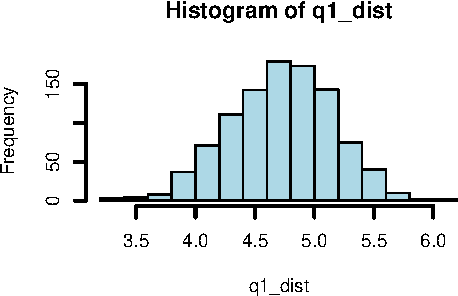
\includegraphics[width=\textwidth,keepaspectratio=true]{005-one-sample-mean-solutions_files/figure-latex/unnamed-chunk-3-1} \end{center}

\begin{Shaded}
\begin{Highlighting}[]
\FunctionTok{round}\NormalTok{(}\FunctionTok{quantile}\NormalTok{(q1\_dist, }\AttributeTok{probs =} \FunctionTok{c}\NormalTok{(}\FloatTok{0.001}\NormalTok{, }\FloatTok{0.005}\NormalTok{, .}\DecValTok{025}\NormalTok{, }\FloatTok{0.05}\NormalTok{, }
                                                 \FloatTok{0.90}\NormalTok{, }\FloatTok{0.95}\NormalTok{, }\FloatTok{0.975}\NormalTok{, }\FloatTok{0.99}\NormalTok{)),}\DecValTok{2}\NormalTok{)}
\end{Highlighting}
\end{Shaded}

\begin{ShadedResult}
\begin{verbatim}
#  0.1% 0.5% 2.5%   5%  90%  95%  98%  99% 
#   3.3  3.6  3.9  4.0  5.2  5.4  5.5  5.7
\end{verbatim}
\end{ShadedResult}

The 95\% Bootstrap interval is given by {[}3.86, 5.54{]} kg. Very
similar to the interval given in part a). Gives us some more confidence
that the CLT has indeed kicked in.

\begin{enumerate}
\def\labelenumi{\alph{enumi}.}
\setcounter{enumi}{2}
\tightlist
\item
  Convert the units of the mean weight gain and 95\% confidence interval
  to pounds. Note that 1 kilogram is equal to 2.2 pounds. Test the null
  hypothesis that the mean weight gain is 16 lbs. State your assumptions
  and justify your choice of test. Be sure to specify the null and
  alternative hypotheses. What do you conclude? We convert the Bootsrap
  CI by simply multiplying the upper and lower limits by 2.2lbs to give:
\end{enumerate}

\begin{Shaded}
\begin{Highlighting}[]
\FunctionTok{quantile}\NormalTok{(q1\_dist, }\AttributeTok{probs =} \FunctionTok{c}\NormalTok{(.}\DecValTok{025}\NormalTok{, }\FloatTok{0.975}\NormalTok{)) }\SpecialCharTok{*} \FloatTok{2.2}
\end{Highlighting}
\end{Shaded}

\begin{ShadedResult}
\begin{verbatim}
#  2.5%  98% 
#   8.5 12.2
\end{verbatim}
\end{ShadedResult}

The null hypothesis is that the theory of weight gain is the same as the
measured weigth gain, \(H_0: \mu = \mu_o = 16\) lbs, and the alternative
hypothesis is \(H_a: \mu \neq 16\) lbs (two tailed test). I want to test
it using the bootstrap method beacause I don't want to assume that the
CLT has kicked in and the sampling distribution is normal. Since the
upper limit of the confidence interval is below 16 lbs, there is
evidence to suggest that we should reject the null hypothesis, i.e., the
actual weight gain might be lower than the theory says.

\newpage

\hypertarget{attitudes-toward-school}{%
\section{Attitudes toward school}\label{attitudes-toward-school}}

The Survey of Study Habits and Attitudes (SSHA) is a psychological test
that measures the motivation, attitude toward school, and study habits
of students. Scores range from 0 to 200. The mean score for U.S. college
students is about 115, and the standard deviation is about 30. A teacher
who suspects that older students have better attitudes toward school
gives the SSHA to 25 students who are at least 30 years of age. Their
mean score is \(\bar{y}\) = 132.2 with a sample standard deviation
\(s = 28\).

\begin{enumerate}
\def\labelenumi{\alph{enumi}.}
\tightlist
\item
  The teacher asks you to carry out a formal statistical test for her
  hypothesis. Perform a test, provide a 95\% confidence interval and
  state your conclusion clearly.
\end{enumerate}

\hypertarget{using-the-t-procedure}{%
\subsection{Using the t procedure}\label{using-the-t-procedure}}

The null hypothesis is that older student mean SSHA score equals all
student mean SSHA scores, \(H_0: \mu = \mu_0 = 115\). The alternate
hypothesis is that older student mean SSHA score is greater than 115,
\(H_a: \mu > 115\) (ie: one-tail test). The sample size is on the
smaller side (ie: below 30), so I chose to use a one sample t-test
because I don't trust the sample sd to be a good estimate of the
population sd. A two tailed 95\% CI is {[}120.64, 143.76{]}. Based on
this, I reject the null hypothesis, .i.e. , our data provides evidence
that there might be a difference in SSHA scores between older students
and the general population of students.

\hypertarget{using-the-z-procedure}{%
\subsection{Using the z procedure}\label{using-the-z-procedure}}

\begin{Shaded}
\begin{Highlighting}[]
\FunctionTok{qnorm}\NormalTok{(}\AttributeTok{p =} \FunctionTok{c}\NormalTok{(}\FloatTok{0.025}\NormalTok{, }\FloatTok{0.975}\NormalTok{), }\AttributeTok{mean =} \FloatTok{132.2}\NormalTok{, }\AttributeTok{sd =} \DecValTok{30}\SpecialCharTok{/}\FunctionTok{sqrt}\NormalTok{(}\DecValTok{25}\NormalTok{))}
\end{Highlighting}
\end{Shaded}

\begin{ShadedResult}
\begin{verbatim}
#  [1] 120 144
\end{verbatim}
\end{ShadedResult}

\begin{Shaded}
\begin{Highlighting}[]
\CommentTok{\# alternatively}
\FloatTok{132.2} \SpecialCharTok{+} \FunctionTok{qnorm}\NormalTok{(}\AttributeTok{p =} \FunctionTok{c}\NormalTok{(}\FloatTok{0.025}\NormalTok{, }\FloatTok{0.975}\NormalTok{)) }\SpecialCharTok{*} \DecValTok{30}\SpecialCharTok{/}\FunctionTok{sqrt}\NormalTok{(}\DecValTok{25}\NormalTok{)}
\end{Highlighting}
\end{Shaded}

\begin{ShadedResult}
\begin{verbatim}
#  [1] 120 144
\end{verbatim}
\end{ShadedResult}

Assuming that the standard deviation of the all U.S. college students of
30 is accurate and taken as sigma, the 95\% confidence interval for the
population mean SSHA score is {[}120.44, 143.96{]}.

\begin{enumerate}
\def\labelenumi{\alph{enumi}.}
\setcounter{enumi}{1}
\tightlist
\item
  What assumptions did you use in part (a). Which of these assumptions
  is most important to the validity of your conclusion in part (a).
\end{enumerate}

We are assuming that this is a simple random sample of older students.
If using the \(t\)-distribution, we are assuming that the standard
deviation of the population is not a good estimate of the standard
deviation of our sample. The most important assumption we've made is
that the CLT has kicked in and therefore the sampling distribution is
normal.

If using \(z\) procedure \(\to\) that the standard deviation of the all
U.S. college students of 30 is accurate and taken as sigma, and that the
sample size is enough that the CLT has kicked in.

\hypertarget{does-a-full-moon-affect-behavior}{%
\section{Does a full moon affect
behavior?}\label{does-a-full-moon-affect-behavior}}

Many people believe that the moon influences the actions of some
individuals. A study of dementia patients in nursing homes recorded
various types of disruptive behaviors every day for 12 weeks. Days were
classified as moon days if they were in a 3-day period centered at the
day of the full moon. For each patient, the average number of disruptive
behaviors was computed for moon days and for all other days. The
hypothesis is that moon days will lead to more disruptive behavior. We
look at a data set consisting of observations on 15 dementia patients in
nursing homes (available in the \texttt{fullmoon.csv} file):

\begin{Shaded}
\begin{Highlighting}[]
\NormalTok{fullmoon }\OtherTok{\textless{}{-}} \FunctionTok{read.csv}\NormalTok{(}\StringTok{"fullmoon.csv"}\NormalTok{)}
\end{Highlighting}
\end{Shaded}

\begin{ShadedResult}
\begin{verbatim}
#     patient moon_days other_days
#  1        1      3.33       0.27
#  2        2      3.67       0.59
#  3        3      2.67       0.32
#  4        4      3.33       0.19
#  5        5      3.33       1.26
#  6        6      3.67       0.11
#  7        7      4.67       0.30
#  8        8      2.67       0.40
#  9        9      6.00       1.59
#  10      10      4.33       0.60
#  11      11      3.33       0.65
#  12      12      0.67       0.69
#  13      13      1.33       1.26
#  14      14      0.33       0.23
#  15      15      2.00       0.38
\end{verbatim}
\end{ShadedResult}

\begin{enumerate}
\def\labelenumi{\alph{enumi}.}
\tightlist
\item
  Calculate a 95\% confidence interval for the mean difference in
  disruptive behaviors. State the assumptions you used to calculate this
  interval.
\end{enumerate}

\begin{Shaded}
\begin{Highlighting}[]
\NormalTok{(moon.mean }\OtherTok{\textless{}{-}} \FunctionTok{mean}\NormalTok{(moon.diff))}
\end{Highlighting}
\end{Shaded}

\begin{ShadedResult}
\begin{verbatim}
#  [1] 2.4
\end{verbatim}
\end{ShadedResult}

\begin{Shaded}
\begin{Highlighting}[]
\NormalTok{(moon.sdev }\OtherTok{\textless{}{-}} \FunctionTok{sd}\NormalTok{(moon.diff))}
\end{Highlighting}
\end{Shaded}

\begin{ShadedResult}
\begin{verbatim}
#  [1] 1.5
\end{verbatim}
\end{ShadedResult}

\begin{Shaded}
\begin{Highlighting}[]
\NormalTok{(moon.n }\OtherTok{\textless{}{-}} \FunctionTok{length}\NormalTok{(moon.diff))}
\end{Highlighting}
\end{Shaded}

\begin{ShadedResult}
\begin{verbatim}
#  [1] 15
\end{verbatim}
\end{ShadedResult}

\begin{Shaded}
\begin{Highlighting}[]
\FunctionTok{qt\_scaled}\NormalTok{(}\AttributeTok{p=}\FunctionTok{c}\NormalTok{(}\FloatTok{0.025}\NormalTok{, }\FloatTok{0.975}\NormalTok{), }\AttributeTok{df =}\NormalTok{ moon.n }\SpecialCharTok{{-}} \DecValTok{1}\NormalTok{, }\AttributeTok{mean =}\NormalTok{ moon.mean, }\AttributeTok{sd =}\NormalTok{ moon.sdev}\SpecialCharTok{/}\FunctionTok{sqrt}\NormalTok{(moon.n))}
\end{Highlighting}
\end{Shaded}

\begin{ShadedResult}
\begin{verbatim}
#  [1] 1.6 3.2
\end{verbatim}
\end{ShadedResult}

\begin{Shaded}
\begin{Highlighting}[]
\CommentTok{\# alternatively}
\NormalTok{moon.mean }\SpecialCharTok{+} \FunctionTok{qt}\NormalTok{(}\AttributeTok{p =} \FunctionTok{c}\NormalTok{(}\FloatTok{0.025}\NormalTok{, }\FloatTok{0.975}\NormalTok{), }\AttributeTok{df =}\NormalTok{ moon.n }\SpecialCharTok{{-}} \DecValTok{1}\NormalTok{) }\SpecialCharTok{*}\NormalTok{ moon.sdev}\SpecialCharTok{/}\FunctionTok{sqrt}\NormalTok{(moon.n)}
\end{Highlighting}
\end{Shaded}

\begin{ShadedResult}
\begin{verbatim}
#  [1] 1.6 3.2
\end{verbatim}
\end{ShadedResult}

Assuming a simple random sample and that our sample is representative of
the population, and that the difference in distruptive events is
normally distributed in the population (OR you can say that you believe
the Central Limit Theorem (CLT) has kicked in), I calculated a 95\%
confidence interval for the population mean difference of {[}1.62, 3.24
distruptive events on full moon days when compared to other days. This
was done using the \(t\) procedure due to the unknown sigma and small
sample size of n = 15.

\begin{enumerate}
\def\labelenumi{\alph{enumi}.}
\setcounter{enumi}{1}
\tightlist
\item
  Test the hypothesis that moon days will lead to more disruptive
  behavior. State your assumptions and provide a brief conclusion based
  on your analysis.
\end{enumerate}

\begin{Shaded}
\begin{Highlighting}[]
\CommentTok{\#t{-}statistic}
\NormalTok{(t\_statistic }\OtherTok{\textless{}{-}}\NormalTok{ (moon.mean }\SpecialCharTok{{-}} \DecValTok{0}\NormalTok{) }\SpecialCharTok{/}\NormalTok{ (moon.sdev}\SpecialCharTok{/}\FunctionTok{sqrt}\NormalTok{(moon.n)))}
\end{Highlighting}
\end{Shaded}

\begin{ShadedResult}
\begin{verbatim}
#  [1] 6.5
\end{verbatim}
\end{ShadedResult}

\begin{Shaded}
\begin{Highlighting}[]
\CommentTok{\# p{-}value}
\FunctionTok{pt}\NormalTok{(}\AttributeTok{q =}\NormalTok{ t\_statistic, }\AttributeTok{df =}\NormalTok{ moon.n}\DecValTok{{-}1}\NormalTok{, }\AttributeTok{lower.tail =}\NormalTok{ F)}
\end{Highlighting}
\end{Shaded}

\begin{ShadedResult}
\begin{verbatim}
#  [1] 7.6e-06
\end{verbatim}
\end{ShadedResult}

\(H_0: \mu = 0\) (i.e.~that there is no difference in distruptive
behaviours on full moon nights when compared to other nights) and
\(H_a: \mu > 0\) (i.e.~that there are more distruptive behaviours on
full moon nights when compared to other nights).

I calculate a one-sided (to the right) p-value using the \(t\) statistic
(because unknown sigma and small sample size of n = 15) of
\ensuremath{7.59\times 10^{-6}}. Assuming the null hyposthesis is true,
there is very small probability that the observed mean difference of
2.43 came from the null distribution. We could also say that since
\(\mu = 0\) is not contained within our 95\% confidence interval, this
provides evidence against the null hypothesis. This is based on the
assumptions that the sample distribution here is enough that the CLT has
kicked in as well.

\begin{enumerate}
\def\labelenumi{\alph{enumi}.}
\setcounter{enumi}{2}
\tightlist
\item
  Find the minimum value of the mean difference in disruptive behaviors
  (\(\bar{y}\)) needed to reject the null hypothesis.
\end{enumerate}

We first need to figure out for what values we can reject the null.
Since this is a one-sided alternative we want and \(\alpha=0.05\) in the
right tail. The cutoff is then given by:

\begin{Shaded}
\begin{Highlighting}[]
\NormalTok{(tscore.null }\OtherTok{\textless{}{-}} \FunctionTok{qt}\NormalTok{(}\AttributeTok{p =} \FloatTok{0.95}\NormalTok{, }\AttributeTok{df =} \DecValTok{15{-}1}\NormalTok{))}
\end{Highlighting}
\end{Shaded}

\begin{ShadedResult}
\begin{verbatim}
#  [1] 1.8
\end{verbatim}
\end{ShadedResult}

Then we solve for \(\bar{y}\) in the \(t\)-statistic formula:

\begin{align*}
t_{statistic} & = \frac{\bar{y} - \mu_0}{s/\sqrt{n}} \\
1.76 & = \frac{\bar{y} - 0}{1.46/\sqrt{15}}
\end{align*}

The solution to the above equation is:

\begin{Shaded}
\begin{Highlighting}[]
\NormalTok{tscore.null}\SpecialCharTok{*}\NormalTok{(moon.sdev}\SpecialCharTok{/}\FunctionTok{sqrt}\NormalTok{(moon.n))}
\end{Highlighting}
\end{Shaded}

\begin{ShadedResult}
\begin{verbatim}
#  [1] 0.66
\end{verbatim}
\end{ShadedResult}

Assuming \(H_0\) is true, under the null distribution the minimum value
in mean difference in distruptive behaviours needed to reject the null
hypothesis at an \(\alpha=0.05\) level is 0.66 distruptive behaviours.

\begin{enumerate}
\def\labelenumi{\alph{enumi}.}
\setcounter{enumi}{3}
\tightlist
\item
  What is the probability of detecting an increase of 1.0 aggressive
  behavior per day during moon days?
\end{enumerate}

\[
H_0: \mu = 0 \qquad \qquad H_A: \mu > 1
\] This is a standard power calculation. In the first step, we calculate
the difference in mean disruptive behaviours needed to reject the null
hypothesis, which we calculated in part c) to be 0.66. The corresponding
\(t\) value under the alternative hypothesis distribution is given by

\begin{align*}
t_{statistic} & = \frac{\bar{y} - \mu_A}{s/\sqrt{n}} \\
 & = \frac{0.664 - 1}{1.46/\sqrt{15}} \\
 & = -0.890
\end{align*}

We then calculate the probability of observing this value or more under
the alternative hypothesis distribution:

\begin{Shaded}
\begin{Highlighting}[]
\FunctionTok{pt}\NormalTok{(}\AttributeTok{q =} \SpecialCharTok{{-}}\FloatTok{0.890}\NormalTok{, }\AttributeTok{df =}\NormalTok{ moon.n }\SpecialCharTok{{-}} \DecValTok{1}\NormalTok{, }\AttributeTok{lower.tail =} \ConstantTok{FALSE}\NormalTok{)}
\end{Highlighting}
\end{Shaded}

\begin{ShadedResult}
\begin{verbatim}
#  [1] 0.81
\end{verbatim}
\end{ShadedResult}

Therefore, the power to detect an increase of 1.0 aggressive behavior
per day during moon days is 80.57\%.

%\showmatmethods


\bibliography{pinp}
\bibliographystyle{jss}



\end{document}
